% !TEX root = ../../../main.tex

\toggletrue{image}
\togglefalse{imagehover}
\chapterimage{logic_gatter_joke}
\chapterimagetitle{\uppercase{Hamlet}}
\chapterimageurl{William Shakespeare}
\toggletrue{imagehover}

\chapter{Grundgatter}
\label{chapter-grundgatter}

Die Grundlage aller Computerbauteile bilden die \textbf{Logikgatter} (engl. logic gates). Ein Logikgatter ist eine elektronische Schaltung. Es gibt \textbf{drei Grundgatter}, aus denen alle anderen Bauteile bestehen. Die Lernziele lauten: \\

\newcommand{\grundgatterLernziele}{
\protect\begin{minipage}{\textwidth}
\begin{todolist}
\item Sie erklären, was wir unter einem Logikgatter verstehen.
\item Sie erklären an einem Beispiel das Verhalten der drei Logikgatter \texttt{UND}, \texttt{ODER} und \texttt{NICHT}.
\item Sie stellen die drei Logikgatter \texttt{UND}, \texttt{ODER} und \texttt{NICHT} grafisch dar.
\end{todolist}
\end{minipage}
}

\lernziel{\autoref{chapter-grundgatter}, \nameref{chapter-grundgatter}}{\protect\grundgatterLernziele}

\grundgatterLernziele

\section{\texttt{UND}-Gatter}

Das \texttt{UND}-Gatter (eng. \texttt{AND}-Gate\footnote{Gatter (bzw. Gate) ist die Abkürzung für Logikgatter bzw. Logic Gate.}) besitzt das Verhalten, dass die Glühbirne nur dann leuchtet, wenn \textbf{beide Schalter} gedrückt sind (siehe \autoref{logicly-and}).

\begin{figure}[htb]
\centering
\begin{minipage}{0.225\textwidth}
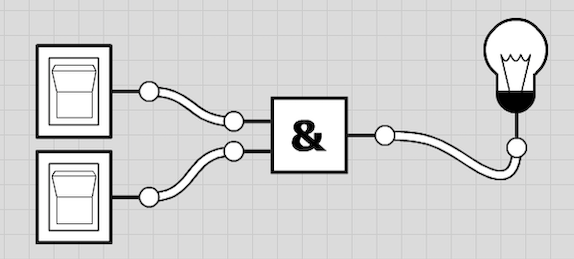
\includegraphics[width=\textwidth]{./and/and_off_off}
\end{minipage}
\begin{minipage}{0.225\textwidth}
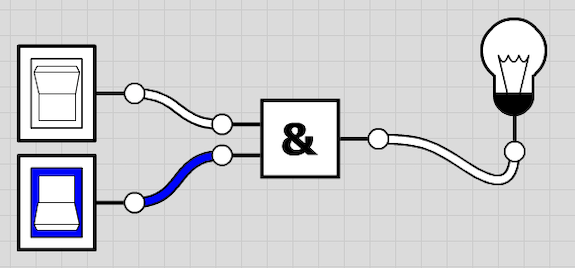
\includegraphics[width=\textwidth]{./and/and_off_on}
\end{minipage}
\begin{minipage}{0.225\textwidth}
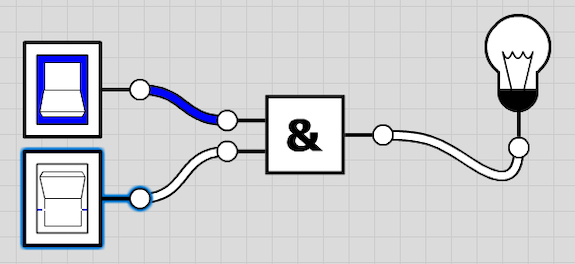
\includegraphics[width=\textwidth]{./and/and_on_off}
\end{minipage}
\begin{minipage}{0.225\textwidth}
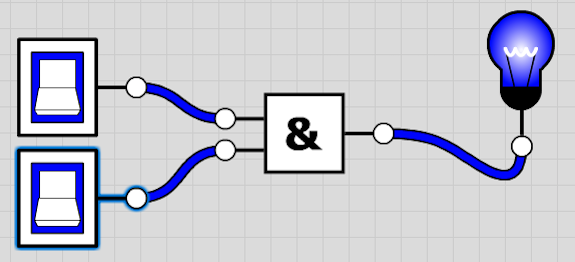
\includegraphics[width=\textwidth]{./and/and_on_on}
\end{minipage}
\caption{Es gibt vier Kombinationen, wie die Schalter betätigt werden können \cite{bowlerhat2023logicly}.}
\label{logicly-and}
\end{figure}

Wenn wir die Bauteile von Hand zeichnen, dann ist es einfacher, wenn wir Schalter und Glühbirnen nicht zeichnen müssen. Wir bezeichnen die Schalter als \textbf{Eingänge} und die Glühbirne als \textbf{Ausgang}. Das \texttt{UND}-Gatter aus \autoref{logicly-and} hat \textbf{zwei Eingänge}. Wir kürzen einen Eingang mit $E$ ab und geben jedem Eingang eine Nummer. Ausserdem hat das Gatter \textbf{einen Ausgang}. Wir kürzen dies mit $A_0$ ab. \autoref{circuit-and} zeigt die kompakte Darstellung, die in der Digitaltechnik geläufig ist.

\begin{figure}[htb]
\centering
\begin{circuitikz}
\draw (0,0) node[and port] (AND1) {}
(AND1.in 1) node[anchor=east] {$E_0$} 
(AND1.in 2) node[anchor=east] {$E_1$}
(AND1.out) node[anchor=west] {$A_0$};
\end{circuitikz}
\caption{Das \texttt{UND}-Gatter besteht aus einem Rechteck mit einem \protect\say{Kaufmanns-Und} (eng. ampersand) darin. Die Eingänge werden immer links vom Bauteil gezeichnet, die Ausgänge rechts.}
\label{circuit-and}
\end{figure}

Wir können die Funktionsweise des \texttt{UND}-Gatters auch gut mithilfe eines Schaltplans der Elektrotechnik veranschaulichen (siehe \autoref{circuit-and-schaltplan}). Die Glühbirne leuchtet nur dann, wenn sowohl Schalter $E_0$ als auch Schalter $E_1$ gedrückt sind. Die Schalter sind sogenannte Schliesser. Wenn Sie gedrückt sind, dann ist der Stromkreis geschlossen. Dann kann von der Batterie aus der Strom in Pfeilrichtung fliessen und die Glühbirne leuchten.

\begin{figure}[htb]
\centering
\begin{circuitikz}
\draw (0,0) to (1,0) to[cute open switch, label=$E_0$] (2.5,0) to (3.5,0) to[cute open switch, label=$E_1$] (5.5,0)
to (5.5, -1) to[lamp, label=$A_0$] (2.5, -1) to[battery1=\SI{5}{V}] (0,-1) to (0,0);
\end{circuitikz}
\caption{Zwei Schalter ($E_0$ und $E_1$), eine Batterie (Spannungsquelle) und eine Lampe ($A_0$).}
\label{circuit-and-schaltplan}
\end{figure}

\section{\texttt{ODER}-Gatter}

Das \texttt{ODER}-Gatter (eng. \texttt{OR}-Gate) besitzt das Verhalten, dass die Glühbirne nur dann leuchtet, wenn \textbf{mindestens} ein Schalter gedrückt ist (siehe \autoref{logicly-or}).

\begin{figure}[htb]
\centering
\begin{minipage}{0.225\textwidth}
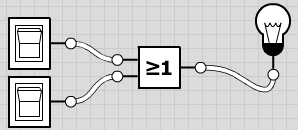
\includegraphics[width=\textwidth]{./or/or_off_off}
\end{minipage}
\begin{minipage}{0.225\textwidth}
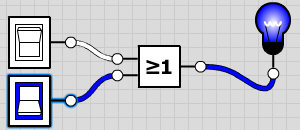
\includegraphics[width=\textwidth]{./or/or_off_on}
\end{minipage}
\begin{minipage}{0.225\textwidth}
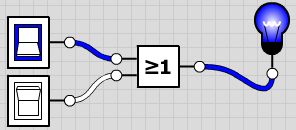
\includegraphics[width=\textwidth]{./or/or_on_off}
\end{minipage}
\begin{minipage}{0.225\textwidth}
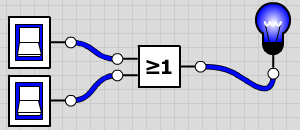
\includegraphics[width=\textwidth]{./or/or_on_on}
\end{minipage}
\caption{Es dürfen auch beide Schalter gedrückt sein.}
\label{logicly-or}
\end{figure}

Wir zeichnen das \texttt{ODER}-Gatter (siehe \autoref{circuit-or}) mit zwei Eingängen und einem Ausgang.

\begin{figure}[htb]
\centering
\begin{circuitikz}
\draw (0,0) node[or port] (OR1) {}
(OR1.in 1) node[anchor=east] {$E_0$} 
(OR1.in 2) node[anchor=east] {$E_1$}
(OR1.out) node[anchor=west] {$A_0$};
\end{circuitikz}
\caption{Das \texttt{ODER}-Gatter: Rechteck mit Grösser-Gleich-Zeichen ($\geq$) und einer \num{1} darin.}
\label{circuit-or}
\end{figure}

Die Funktionsweise des \texttt{ODER}-Gatters ist in \autoref{circuit-or-schaltplan} als Schaltplan veranschaulicht.

\begin{figure}[H]
\centering
\begin{circuitikz}
\draw (0,0) to (1,0) to (1, 0.5) to (2, 0.5) to[cute open switch, label=$E_0$] (3.5, 0.5) to (4, 0.5) to (4, 0);
\draw (0,0) to (1,0) to (1, -0.75) to (2, -0.75) to[cute open switch, label=$E_1$] (3.5, -0.75) to (4, -0.75) to (4, 0);
\draw (4,0) to (5.5, 0) to (5.5, -1.5) to[lamp, label=$A_0$] (2.5, -1.5) to[battery1=\SI{5}{V}] (0,-1.5) to (0,0);
\end{circuitikz}
\caption{Ein Schalter muss mindestens gedrückt sein, damit die Lampe leuchtet.}
\label{circuit-or-schaltplan}
\end{figure}

\section{\texttt{NICHT}-Gatter}

Das \texttt{NICHT}-Gatter (eng. \texttt{NOT}-Gate) besitzt das Verhalten, dass die Glühbirne nur dann leuchtet, wenn der Schalter \textbf{nicht} gedrückt ist (siehe \autoref{logicly-not}).

\begin{figure}[H]
\centering
\begin{minipage}{0.25\textwidth}
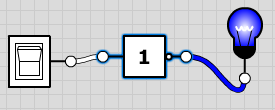
\includegraphics[width=\textwidth]{./not/not_off}
\end{minipage}
\begin{minipage}{0.25\textwidth}
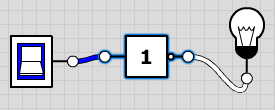
\includegraphics[width=\textwidth]{./not/not_on}
\end{minipage}
\caption{Das \texttt{NICHT}-Gatter besitzt nur einen Eingang.}
\label{logicly-not}
\end{figure}

Das \texttt{NICHT}-Gatter \say{dreht} den Strom quasi um. Wir nennen dieses Gatter auch deshalb \textbf{Inverter}\footnote{Invertieren bedeutet umkehren beziehungsweise umdrehen.}. Wir zeichnen das Gatter mit \textbf{einem} Eingang und \textbf{einem} Ausgang (siehe \autoref{circuit-not}).

\begin{figure}[ht]
\centering
\begin{minipage}{0.45\textwidth}
\centering
\begin{circuitikz}
\draw (0,0) node[european not port] (NOT1) {}
(NOT1.in) node[anchor=east] {$E_0$} 
(NOT1.out) node[anchor=west] {$A_0$};
\end{circuitikz}
\caption{\texttt{NICHT}-Gatter: ausserhalb des Rechtecks wird ein Kreis gezeichnet.}
\label{circuit-not}
\end{minipage}
\hfill
\begin{minipage}{0.45\textwidth}
\centering
\begin{circuitikz}
\draw (0,0) node[buffer port] (BUFFER1) {}
(BUFFER1.in 1) node[anchor=east] {$E_0$} 
(BUFFER1.out) node[anchor=west] {$A_0$};
\end{circuitikz}
\caption{\texttt{BUFFER}-Gatter: besteht aus einem Rechteck mit einer \num{1} darin.}
\label{circuit-buffer}
\end{minipage}
\end{figure}

Die Darstellung des \texttt{NICHT}-Gatters können wir uns besser vorstellen, wenn wir zunächst das \texttt{BUFFER}-Gatter betrachten. Das \texttt{BUFFER}-Gatter leitet den Strom einfach unverändert weiter. Der Kreis beim \texttt{NICHT}-Gatter symbolisiert das \protect\say{Umdrehen} des Stroms.

Die Funktionsweise des \texttt{NICHT}-Gatters ist in \autoref{circuit-not-schaltplan} als Schaltplan veranschaulicht. Der Schalter $E_0$ ist ein sogenannter Öffner. Wenn der Öffner gedrückt ist, dann ist der Stromkreis unterbrochen. Nur wenn der Öffner \textbf{nicht} gedrückt ist, kann von der Batterie aus der Strom in Pfeilrichtung fliessen und die Glühbirne leuchten.

\begin{figure}[htb]
\centering
\begin{circuitikz}
\draw (0,0) to (1,0) to[normal closed switch, label=$E_0$] (2.5,0) to (3.5,0) to (5.5,0)
to (5.5, -1) to[lamp, label=$A_0$] (2.5, -1) to[battery1=\SI{5}{V}] (0,-1) to (0,0);
\end{circuitikz}
\caption{Der Öffner wird betätigt (man drückt von unten gegen den Schalter) und dadurch wird der Stromkreis unterbrochen.}
\label{circuit-not-schaltplan}
\end{figure}

\vspace{-0.5cm}

\section{Übungen}

\begin{exercise}\label{uebung-raum}
Oft hat es für das in Licht in einem Raum mehrere Schalter. In \autoref{figure-logikgatter-uebung-oder} gibt es zwei Schalter, welch das Licht einschalten können. Tragen Sie für diese Situation das passende Logikgatter ein.

\begin{figure}[htb]
\centering
\begin{minipage}{0.45\textwidth}
\centering
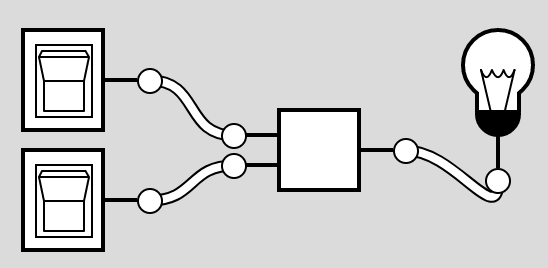
\includegraphics[height=2cm]{logikgatter_uebung_oder}
\caption{Übung \ref{uebung-raum}}
\label{figure-logikgatter-uebung-oder}
\end{minipage}
\hfill
\begin{minipage}{0.45\textwidth}
\centering
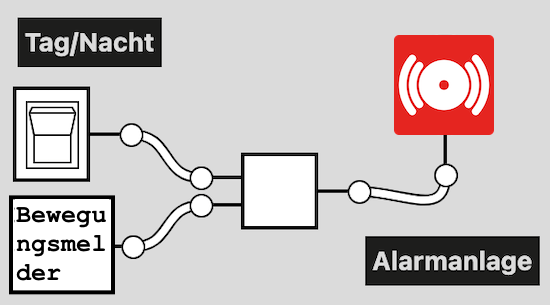
\includegraphics[height=2cm]{logikgatter_uebung_und}
\caption{Übung \ref{uebung-sensor}}
\label{figure-logikgatter-uebung-und}
\centering
\end{minipage}
\end{figure}
\end{exercise}

\vspace{-0.75cm}

\begin{exercise}\label{uebung-sensor}
In einem Museum gibt es einen Bewegungssensor (siehe \autoref{figure-logikgatter-uebung-und}). Der Sensor soll nur in der Nacht einen Alarm auslösen. Dazu stellt der Nachtwächter mit einem Schalter das Überwachungssystem \say{scharf}. Tragen Sie für diese Situation das passende Logikgatter ein.
\end{exercise}

\begin{exercise}
Finden Sie ein Alltagsbeispiel für das \texttt{NICHT}-Gatter. Beschreiben Sie die Situation.

% Die Kronjuwelen liegen auf einem Gewichtssensor. Wenn man die Kronjuwelen wegnimmt, dann soll ein Alarm ertönen. Dafür kann man ein NICHT-Gatter verwenden. Wenn der Gewichtssensor kein Gewicht ermittelt, dann ertönt der Alarm.

\fillwithgrid{\stretch{1}}
\end{exercise}
